\let\negmedspace\undefined
\let\negthickspace\undefined
\documentclass[journal]{IEEEtran}
\usepackage[a5paper, margin=10mm, onecolumn]{geometry}
%\usepackage{lmodern} % Ensure lmodern is loaded for pdflatex
\usepackage{tfrupee} % Include tfrupee package

\setlength{\headheight}{1cm} % Set the height of the header box
\setlength{\headsep}{0mm}     % Set the distance between the header box and the top of the text

\usepackage{gvv-book}
\usepackage{gvv}
\usepackage{cite}
\usepackage{amsmath,amssymb,amsfonts,amsthm}
\usepackage{algorithmic}
\usepackage{graphicx}
\usepackage{float}

\usepackage{textcomp}
\usepackage{xcolor}
\usepackage{txfonts}
\usepackage{listings}
\usepackage{enumitem}
\usepackage{mathtools}
\usepackage{gensymb}
\usepackage{comment}
\usepackage[breaklinks=true]{hyperref}
\usepackage{tkz-euclide} 
\usepackage{listings}
% \usepackage{gvv}                                        
\def\inputGnumericTable{}                                 
\usepackage[latin1]{inputenc}                                
\usepackage{color}                                            
\usepackage{array}                                            
\usepackage{longtable}                                       
\usepackage{calc}                                             
\usepackage{multirow}                                         
\usepackage{hhline}                                           
\usepackage{ifthen}                                           
\usepackage{lscape}
\usepackage{circuitikz}


\renewcommand{\thefigure}{\theenumi}
\renewcommand{\thetable}{\theenumi}
\setlength{\intextsep}{10pt} % Space between text and floats


\numberwithin{equation}{enumi}
\numberwithin{figure}{enumi}
\renewcommand{\thetable}{\theenumi}


% Marks the beginning of the document
\begin{document}
\bibliographystyle{IEEEtran}
\vspace{3cm}

\title{GATE 2022 CH}
\author{EE25BTECH11006 - ADUDOTLA SRIVIDYA}
\maketitle
\noindent
\textbf{Q.1 -- Q.5 Carry ONE mark each}

\vspace{0.5cm}

\begin{enumerate}[start=1, label={Q\arabic*.}]

\item Inhaling the smoke from a burning \underline{\hspace{1.5cm}}could \underline{\hspace{1.5cm}}you quickly.
\begin{enumerate} 
\begin{multicols}{4}
\item tire/tier
\item tire/tyre
\item tyre/tire
\item tyre/tier
  \end{multicols}
  \end{enumerate}
\item A sphere of radius r cm is packed in a box of cubical shape. What should be the minimum volume (in $cm^3$) of the box that can enclose the sphere?
\begin{enumerate} 
\begin{multicols}{4}
\item $r^3/8$
\item $r^3$
\item $2r^3$
\item $8r^3$
  \end{multicols}
  \end{enumerate}
\item Pipes P and Q can fill a storage tank in full with wate in 10 and 6 minutes,respectively.Pipe R draws the water out from the storage tank at arate of $34$ litres per minute. P,Q and R operate at a constant rate.
If it takes one hour to completely empty a full storage tank with all the pipes operating simultaneously, what is the capacity of the storage tank (in litres)?
\begin{enumerate} 
\begin{multicols}{4}
  \item $26.8$
  \item $60.0$
  \item $120.0$
  \item $127.5$
  \end{multicols}
  \end{enumerate}
\item Six persons P,Q,R,S,T and U are sitting around a circular table facing the center not necessarily in the same order. Consider the following statements: \newline
$\bullet$ \; P sits next to S and T.\newline
$\bullet$ \; Q sits diametrically opposite to P.\newline
$\bullet$ \;The shortest distance between S and R is equal to the shortest distance between T and U.\newline
Based on the above statements, Q is a neighbour of 
\begin{enumerate} 
\begin{multicols}{4}
  \item U and S
  \item R and T
  \item R and U
  \item P and S
  \end{multicols}
  \end{enumerate}
\item A building has several rooms and doors as shown in the top view of the building given below. The doors are closed initially. What is the minimum number of doors that need to be opened in order to go from the point P to the point Q?
\begin{figure}[H]
    \centering
    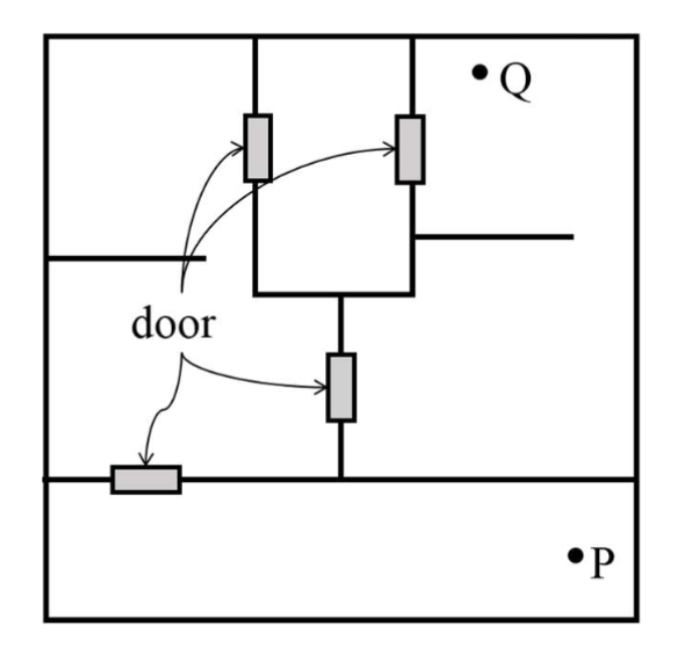
\includegraphics[width=0.5\linewidth]{figs/fig1.jpeg}
    \caption{First fig}
    \label{fig:first}
\end{figure}
\begin{enumerate} 
\begin{multicols}{4}
  \item $4$
  \item $3$
  \item $2$
  \item $1$
  \end{multicols}
  \end{enumerate}
  \vspace{0.5cm}
\item Rice, a versatile and inexpensive source of carbohydrate, is a critical component of diet worldwide. Climate change, causing extreme weather, poses a threat to sustained availability of rice. Scientists are working on developing Green Super Rice (GSR), which is resilient under extreme weather conditions yet gives higher yields sustainably.
Which one of the following is the CORRECT logical inference based on the information given in the above passage?

\begin{enumerate}
    \item GSR is an alternative to regular rice, but it grows only in an extreme weather
    \item GSR may be used in future in response to adverse effects of climate change
    \item GSR grows in an extreme weather, but the quantity of produce is lesser than regular rice
    \item Regular rice will continue to provide good yields even in extreme weather
\end{enumerate}
\vspace{0.5cm}
\item A game consists of spinning an arrow around a stationary disk as shown below. When the arrow comes to rest, there are eight equally likely outcomes. It could come to rest in any one of the sectors numbered $1, 2, 3, 4, 5, 6, 7$ or $8$ as shown.

Two such disks are used in a game where their arrows are independently spun.

What is the probability that the sum of the numbers on the resulting sectors upon spinning the two disks is equal to 8 after the arrows come to rest?
\newpage
\begin{figure}[H]
    \centering
    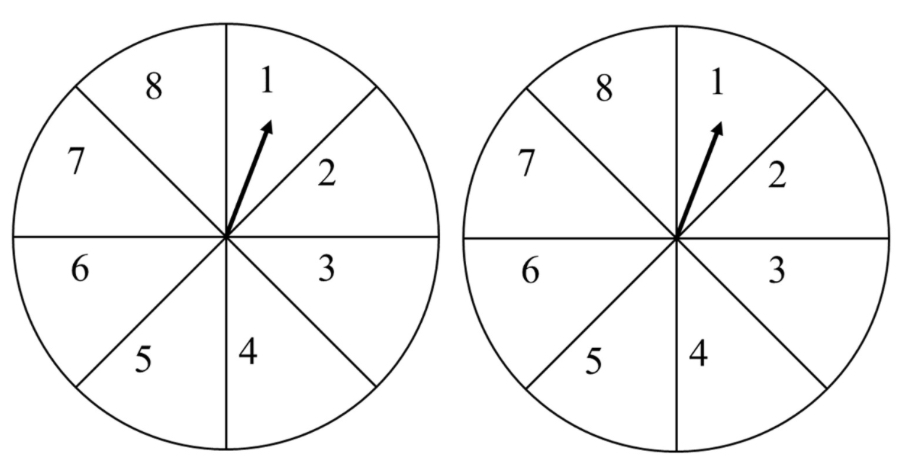
\includegraphics[width=0.8\linewidth]{figs/fig2.jpeg}
    \caption{Sec fig}
    \label{fig:sec}
\end{figure}
\begin{enumerate} 
\begin{multicols}{4}
  \item \[\frac{1}{16}\]
  \item \[\frac{5}{64}\]
  \item \[\frac{3}{32}\]
  \item \[\frac{7}{64}\]
  \end{multicols}
  \end{enumerate}
\item Consider the following inequalities.
(i) $3p-q<4$ (ii) $3q-p<12$\newline
Which one of the following expressions below satisfies the above two inequalities?
\begin{enumerate} 
\begin{multicols}{4}
  \item $p+q<8$
  \item $p+q=8$
  \item .
  \item .
  \end{multicols}
  \end{enumerate}
\item Given below are three statements and four conclusions drawn based on the statements.

Statement 1: Some engineers are writers.

Statement 2: No writer is an actor.

Statement 3: All actors are engineers.

Conclusion I: Some writers are engineers.

Conclusion II: All engineers are actors.

Conclusion III: No actor is a writer.

Conclusion IV: Some actors are writers.

Which one of the following options can be logically inferred?
\begin{enumerate}
\item Only conclusion I is correct
\item Only conclusion II and conclusion III are correct
\item Only conclusion I and conclusion III are correct
\item Either conclusion III or conclusion IV is correct
\end{enumerate}
\newpage
\item Which on of the following sets of pieces can be assembled to form a square with a single round hole near the center? Pieces cannot overlap.
\begin{enumerate}
    \item \begin{figure}[H]
        \centering
        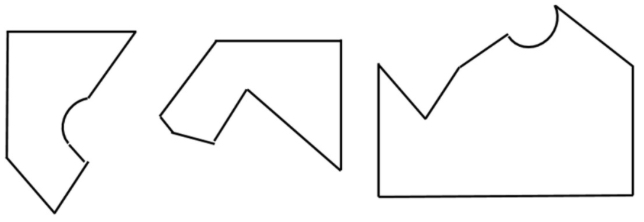
\includegraphics[width=0.5\linewidth]{figs/fig3a.jpeg}
        \caption{3a fig}
        \label{fig:3a}
    \end{figure}
    \item \begin{figure}[H]
        \centering
        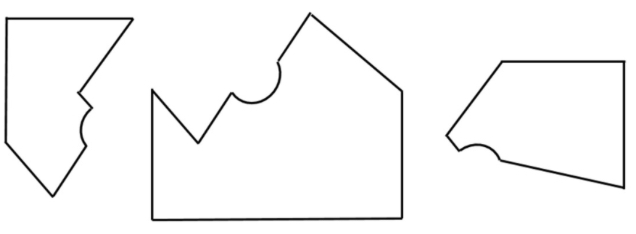
\includegraphics[width=0.5\linewidth]{figs/fig3b.jpeg}
        \caption{3b fig}
        \label{fig:3b}
    \end{figure}
    \item \begin{figure}[H]
        \centering
        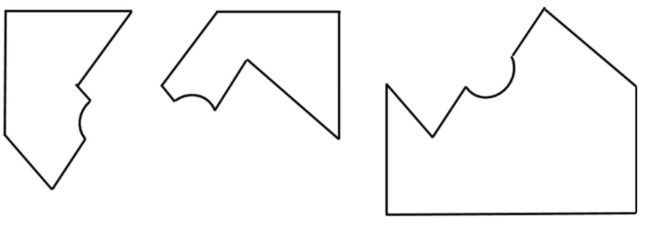
\includegraphics[width=0.5\linewidth]{figs/fig3c.jpeg}
        \caption{3c fig}
        \label{fig:3c}
    \end{figure}
    \item \begin{figure}[H]
        \centering
        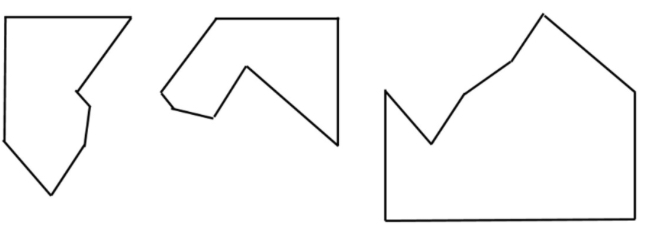
\includegraphics[width=0.5\linewidth]{figs/fig3d.jpeg}
        \caption{3d fig}
        \label{fig:3d}
    \end{figure}
\end{enumerate}
\newpage
\textbf{Q.11 -- Q.35 Carry ONE mark each}

\vspace{0.5cm}
\item The value of $(1+i)^{12}$, where $i=\sqrt{-1}$,is
\begin{enumerate}
\begin{multicols}{4}
    \item $-64i$
    \item $64i$
    \item $64$
    \item $-64$
\end{multicols}
\end{enumerate}
\item Given matrix $A=\begin{bmatrix} x & 1 & 3 \\ y & 2 & 6 \\ 3 & 5 & 7 \end{bmatrix}$,the ordered pair (x,y) for which $det(A)=0$ is
\begin{enumerate}
    \begin{multicols}{4}
        \item $(1,1)$
        \item $(1,2)$
        \item $(2,2)$
        \item $(2,1)$
    \end{multicols}
\end{enumerate}
\item Let $f(x)=e^{-|x|}$,where x is real. The value of $\dfrac{dy}{dx}$ at $x=-1$ is 
\begin{enumerate}
\begin{multicols}{4}
    \item $-e$
    \item $e$
    \item $\dfrac{1}{e}$
    \item $\dfrac{-1}{e}$
\end{multicols}
\end{enumerate}
\item The value of the real variable $x\geq0$,which maximizes the function $f(x)=x^e e^{-x}$ is
\begin{enumerate}
    \begin{multicols}{4}
        \item $e$
        \item $0$
        \item $\dfrac{1}{e}$
        \item $1$
    \end{multicols} 
\end{enumerate}
\item For a single component system at vapor liquid equilibrium,the extensive variables A,V,S and N denote the Helmholtz free energy,volume,entropy and number of moles respectively in a given phase. If superscripts (v) and (l) denote the vapor and liquid phase, respectively, the relation that is NOT CORRECT is
\begin{enumerate} 
\begin{multicols}{2}
  \item $\left( \frac{\partial A^{(l)}}{\partial V^{(l)}} \right)_{T,N^{(l)}}
=\left( \frac{\partial A^{(v)}}{\partial V^{(v)}} \right)_{T,N^{(v)}}$
  \item $\left( \frac{\partial A^{(l)}}{\partial N^{(l)}} \right)_{T,V^{(l)}}
=\left( \frac{\partial A^{(v)}}{\partial N^{(v)}} \right)_{T,V^{(v)}}$
  \item $\left( \frac{A+PV}{N} \right)^{(l)}=\left(\frac{A+PV}{N} \right)^{(v)}$
  \item $\left( \frac{A+TS}{N} \right)^{(l)}=\left(\frac{A+TS}{N} \right)^{(v)}$
  \end{multicols}
  \end{enumerate}
  \item Consider turbulent flow in a pipe under isothermal conditions. Let r denote the radial coordinate and z denote the axial flow direction. On moving away from the wall towards the center of the pipe the rz component of the Reynolds stress
  \begin{enumerate} 
\begin{multicols}{2}
  \item Increases and then decreases
  \item Decreases and then increases
  \item Remains unchanged
  \item Only increases
  \end{multicols}
  \end{enumerate}
  \item Consider two stationary spherical pure water droplets of diameters $d_1$ and $2d_1$. $CO_2$ diffuses into the droplets from the surroundings. If the rate of diffusion of $CO_2$ into the smaller droplet is $W_1$ mol $s^{-1}$, the rate of diffusion of $CO_2$ into the larger droplet is
\begin{enumerate} 
\begin{multicols}{4}
  \item $2W_1$
  \item $4W_1$
  \item $W_1$
  \item $0.5W_1$
  \end{multicols}
  \end{enumerate}
  \newpage
  \item In soap manufacturing, the triglycerides present in oils and fats are hydrolyzed to mainly produce
  \begin{enumerate} 
\begin{multicols}{2}
  \item Fatty acids and glycerol
  \item Glycerol only
  \item Fatty acids only
  \item Glycerol and paraffins
  \end{multicols}
  \end{enumerate}
\item The chemical formula of Glauber's salt, used in the Kraft process, is
  \begin{enumerate} 
\begin{multicols}{2}
  \item $Na_2CO_3.10H_2O$
  \item $Na_2SO_4.2H_2O$
  \item $NaHPO_4.2H_2O$
  \item $Na_2SO_4.10H_2O$
  \end{multicols}
  \end{enumerate}
  \item Catalytic reforming is commonly used in the petroleum industry to improve fuel quality. The undesirable reaction in the catalytic reforming of naphtha is
  \begin{enumerate} 
\begin{multicols}{2}
  \item Hydro cracking of paraffins
  \item Dehydrogenation of naphthenes
  \item Isomerisation of naphthenes
  \item Cyclisation of paraffins
  \end{multicols}
  \end{enumerate}
\item A control system on the jacket side of a reactor is shown in the figure. Pressurized water flows through the jacket to cool the reactor. The heated water flashes in the boiler. The exothermic reaction heat thus generates steam. Fresh boiler feed water (BFW) is added to make up for the loss of water as steam. Assume that all control valves are aid to open. The controller action, 'direct' or 'reverse', is defined with respect to the controller. Select the option that correctly specifies the action of the controllers.
  \begin{figure}[H]
      \centering
      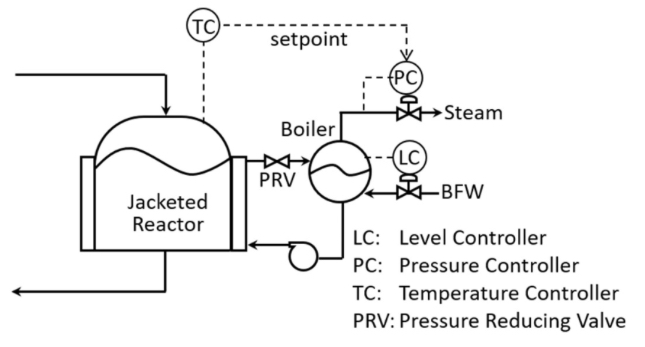
\includegraphics[width=0.5\linewidth]{figs/fig4.jpeg}
      \caption{4}
      \label{fig:fig 4}
  \end{figure}
\begin{enumerate}
\begin{multicols}{2}
    \item PC:Reverse, LC:Direct, TC:Reverse
    \item PC:Direct, LC:Reverse, TC:Direct
    \item PC:Direct, LC:Reverse, TC:Reverse
    \item PC:Reverse, LC:Direct, TC:Direct
\end{multicols}
\end{enumerate}
\newpage
\item Liquid flowing through a heat exchanger (HX) is heated. A bypass stream is provided to control the temperature of the heated exit stream. From the given plumbing options, the one that provides most effective temperature control for large disturbances while avoiding vaporization in the heat exchanger is
\begin{enumerate}
    \item \begin{figure}[H]
        \centering
        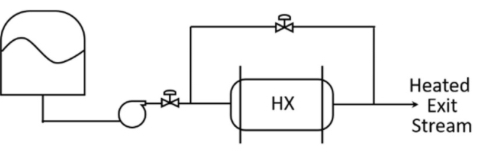
\includegraphics[width=0.5\linewidth]{figs/fig5a.jpeg}
        \caption{5a}
        \label{fig:5a}
    \end{figure}
    \item \begin{figure}[H]
        \centering
        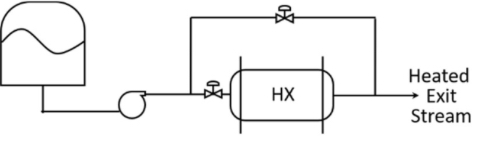
\includegraphics[width=0.5\linewidth]{figs/fig5b.jpeg}
        \caption{5b}
        \label{fig:5b}
    \end{figure}
    \item \begin{figure}[H]
        \centering
        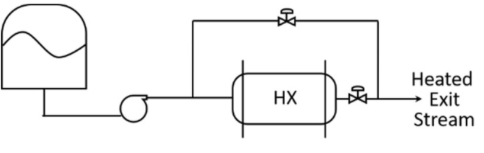
\includegraphics[width=0.5\linewidth]{figs/fig5c.jpeg}
        \caption{5c}
        \label{fig:5c}
    \end{figure}
    \item \begin{figure}[H]
        \centering
        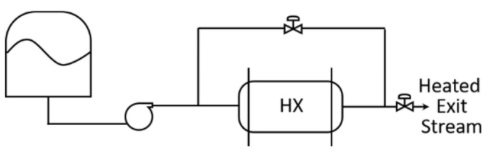
\includegraphics[width=0.5\linewidth]{figs/fig5d.jpeg}
        \caption{5d}
        \label{fig:5d}
    \end{figure}
\end{enumerate}
\newpage
\item The appropriate feedfoorward compensator, $G_{ff}$,in the shown block diagram is
\begin{figure}[H]
    \centering
    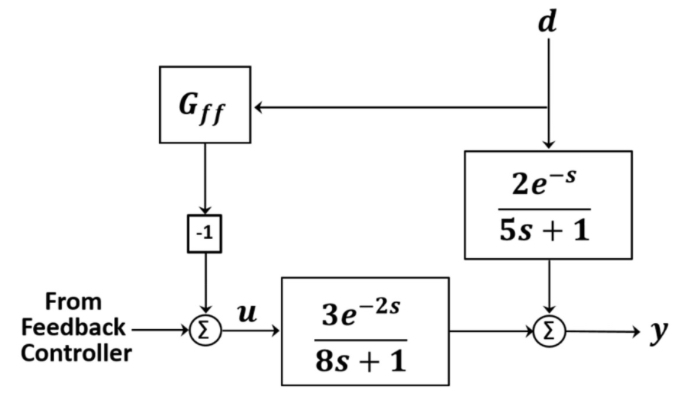
\includegraphics[width=0.5\linewidth]{figs/fig6.jpeg}
    \caption{6}
    \label{fig:6}
\end{figure}
\begin{enumerate} 
\begin{multicols}{2}
  \item $G_{ff}=\dfrac{2}{3} \dfrac{(8s+1)}{(5s+1)}$
  \item $G_{ff}=-\dfrac{2}{3} \dfrac{(8s+1)}{(5s+1)}$
  \item $G_{ff}=\dfrac{3}{2} \dfrac{(5s+1)}{(8s+1)} e^{-s}$
  \item  $G_{ff}=-\dfrac{3}{2} \dfrac{(5s+1)}{(8s+1)} e^{-s}$
  \end{multicols}
  \end{enumerate}
\item Choose the option that correctly pairs the given measurement devices with the quantities they measure.
\begin{center}
\begin{tabular}{c c c c}
\hline
\textbf{S No} & \textbf{Measurement Device} & \textbf{S No} & \textbf{Measured Quantity} \\
\hline
I   & Bourdon Gauge       & A & Temperature   \\
II  & Orifice Plate meter & B & Concentration \\
III & Pyrometer           & C & Pressure      \\
IV  & Colorimeter         & D & Flow rate     \\
\hline
V   & Pirani Gauge        & E & Liquid level  \\
\hline
\end{tabular}
\end{center}
\begin{enumerate} 
\begin{multicols}{2}
  \item I-E II-C III-D IV-B V-A
  \item I-C II-D III-B IV-B V-C
  \item I-C II-D III-E IV-A V-D
  \item I-D II-C III-A IV-E V-C
  \end{multicols}
  \end{enumerate}
\item A simple distillation column is designed to separate an ideal binary mixture to specify distillate and bottom purities at a given column pressure. If $RR_{min}$ is the minimum reflux ratio for this seperation, select the statement that is NOT CORRECT with regard to the variation in total annualized cost (TAC) of the column with reflux ratio (RR).
\begin{enumerate} 
  \item TAC has a minimum with respect to RR
  \item The sharpest rise in TAC occurs as RR approaches $RR_{min}$ from above 
  \item The sharpest decrease in TAC occurs as RR approaches $RR_{min}$ from above
  \item TAC increases with RR for RR>>$RR_{min}$
  \end{enumerate}
\newpage
\item The reaction A $\rightarrow$ B is carried out isothermally on a porous catalyst. The intrinsic reaction rate is $kC^2_A$, where k is the rate constant and $C_A$ is the concentration of A. If the reaction is strongly pore-diffusion controlled, the observed order of the reaction is
\begin{enumerate} 
\begin{multicols}{4}
  \item $1$
  \item $2$
  \item $\dfrac{3}{2}$
  \item $\sqrt{2}$
  \end{multicols}
  \end{enumerate}
\item In an enzymatic reaction,an inhibitor (I) competes with the substrate (S) to bind with the enzyme (E), thereby reducing the rate of product (P) formation. The competitive inhibition follows the reaction mechanism shown below. Let [S] and [I] be the concentration of S and I, respectively, and $r_s$ be the rate of consumption of S. Assuming pseudo-steady state, the correct plot of $\dfrac{1}{-r_s}$ vs $\dfrac{1}{|S|}$ is

$
\begin{aligned}
E + S &\xrightleftharpoons[k_2]{k_1} ES \xrightarrow{k_3} E + P \\
E + I &\xrightleftharpoons[k_{-1}]{k_1} EI
\end{aligned}
$

\begin{enumerate}
\begin{multicols}{2}
\item \begin{figure}[H]
    \centering
    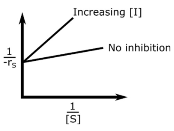
\includegraphics[width=0.4\linewidth]{figs/fig17a.png}
    \caption{Option 1}
\end{figure}

\item \begin{figure}[H]
    \centering
    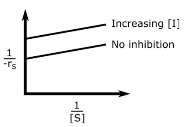
\includegraphics[width=0.4\linewidth]{figs/fig17b.png}
    \caption{Option 2}
\end{figure}

\item \begin{figure}[H]
    \centering
    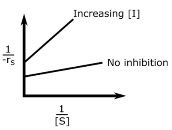
\includegraphics[width=0.4\linewidth]{figs/fig17c.png}
    \caption{Option 3}
\end{figure}

\item \begin{figure}[H]
    \centering
    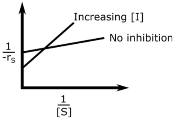
\includegraphics[width=0.4\linewidth]{figs/fig17d.png}
    \caption{Option 4}
\end{figure}
\end{multicols}
\end{enumerate}
\newpage
 
  \item The area of a circular field is $25m^2$. The radius,r, is to be determined using the Newton-Raphson iterative method. For an initial guess of $r=2.500 m$, the revised estimate of r after one iteration is \underline{\hspace{1.5cm}}m (rounded off to three decimal places).
  \vspace{0.2cm}
  \item $5$ moles of liquid benzene, $8$ moles of liquid toluene and $7$ moles of liquid xylene are mixed at $25\degree$C and $1$ bar. Assuming the formation of an ideal solution and using the universal gas constant $R=8.314 J mol^{-1} K^{-1}$, the total entropy change is \underline{\hspace{1.5cm}}$J K^{-1}$ (rounded off to one decimal place).
\vspace{0.2cm}
  \item A perfectly insulated double pipe heat exchanger is operating at steady state. Saturated steam enters the inner pipe at $100\degree$C and leaves as saturated water at $100\degree$C. Cooling water enters the outer pipe at $75\degree$C and exits at $95\degree$C. The overall heat transfer coefficient is $1 KW m^{-2} K^{-1}$ and the heat transfer area is $1m^2$. The average specific heat capacity of water at constant pressure is $4.2kJ kg^{-1} K^{-1}$. The required cooling water flow rate is \underline{\hspace{1.5cm}}kg $s^{-1}$ (rounded off to two decimal places).
  \vspace{0.2cm}
  \item Consider steady-state diffusion in a binary A-B liquid at constant temperature and pressure. The mole-fraction of A at two different locations is $0.8$ and $0.1$. Let $N_{A1}$ be the diffusive flux of A calculated assuming equimolar counter-diffusion. The quantity $\dfrac{(N_{A1} - N_{A2})}{N_{A1}}$X $100$ is \underline{\hspace{1.5cm}} (rounded off to one decimal place).
\vspace{0.2cm}
  \item Consider interphase muss transfer of a species S between two immiscible liquids A and B. The interfacial mass transfer coefficient of S in liquid A is twice of that in liquid B. The equilibrium distribution of S between the liquids is given by $y_S^A=0.5y_S^B$, where $y_S^A$ and $y_S^B$ are the mole-fractions of S in A and B,respectively. The bulk phase mole-fraction of S in A and B is $0.10$ and $0.02$, respectively. If the steady-state flux of S is estimated to be 10 $10 kmol h^{-1}m^{-2}$, the mass transfer coefficient of S in A is \underline{\hspace{1.5cm}} $kmolh^{-1}m^{-2}$ (rounded off to one decimal place).
  \vspace{0.2cm}
  \item A wet solid containing $20\%$ (w/w) moisture (based on mass of bone-dry solid) is dried in a tray-dryer. The critical moisture content of the solid is $10\%$ (w/w). The drying rate (kg $m^{-2}s^{-1}$) is constant for the first $4$ hours, and then decreases linearly to half the initial value in the next $1$ hour. At the end of $5$ hours of drying, the percentage moisture content of the solid is \underline{\hspace{1.5cm}} $\%$(w/w) (rounded off to one decimal place).
  \vspace{0.2cm}
 \item A process described by the transfer function $G_p(s)=\dfrac{(10s+1)}{5s+1}$ is forced by a unit step input at time $t=0$. The output value immediately after the step input (at $t=0^{+}$) is \underline{\hspace{1.5cm}} (rounded off to the nearest integer).
 \vspace{0.2cm}
 \item A compressor with a life of $10$ years costs Rs $10$ lakhs. Its yearly operating cost is Rs $0.5$ lakh. If the annual compound interest rate is $8\%$, the amount needed at present to fund perpetual operation of the compressor is Rs 
 \underline{\hspace{1.5cm}}lakhs (rounded to first decimal place).
 \newpage
 \item The partial differential equation $\dfrac{\partial u}{\partial t}=\dfrac{1}{\pi^{2}} \dfrac{\partial^{2} u}{\partial x^{2}}$ where, $t\geq0$ and $x \in [0,1]$, is subjected to the following initial and boundary conditions:\newline
 $u(x,0=sin(\pi x)$ \newline
 $u(0,t)=0$\newline
 $u(1,t)=0$\newline
 The value of t at which $\dfrac{u(0.5,t)}{u(0.5,0)}=\dfrac{1}{e}$ is 
 \begin{enumerate} 
\begin{multicols}{4}
  \item $1$
  \item $e$
  \item $\pi$
  \item $\dfrac{1}{e}$
  \end{multicols}
  \end{enumerate}
  \item N moles of an ideal gas undergo a two-step process as shown in the figure. Let P, V and T denote the pressure, volume and temperature of the gas, respectively. The gas, initially at state-1 $(P_{1}, V_{1}, T_{1})$ undergoes an isochoric (constant volume) process to reach state-A, and then undergoes an isobaric (constant pressure) expansion to reach state-2 $(P_{2}, V_{2}, T_{2})$ . For an ideal gas, $C_{P} - C_{V} = NR$ where $C_{P}$ and $C_{v}$ are the heat capacities at constant pressure and constant volume, respectively, and assumed to be temperature independent. The heat gained by the gas in the two-step process is given by
\begin{figure}[H]
    \centering
    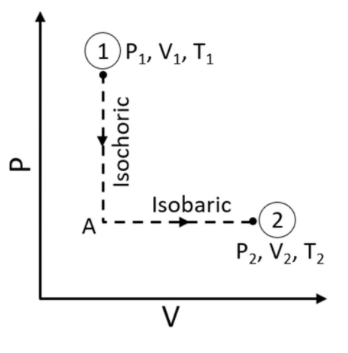
\includegraphics[width=0.3\linewidth]{figs/fig7.jpeg}
    \caption{fig7}
    \label{fig:7}
\end{figure}
\begin{enumerate} 
\begin{multicols}{2}
  \item $P_2(V_2 - V_1) + C_V(T_2 - T_1)$
  \item $P_2(V_2 - V_1) + C_P(T_2 - T_1)$
  \item $C_P(T_2 - T_1) + C_V(T_2 - T_1)$
  \item $P_2V_2 - P_1V_1$
  \end{multicols}
  \end{enumerate}
\vspace{0.2cm}
\item A horizontal cylinder water jet of diameter $D_1=2cm$ strikes a vertical solid plate with a hole of diameter $D_2=1cm$, as shown in the figure. A part of the jet passes through the hole and the rest is deflected along the plate. The density of water is $1000 kg m^{-3}$. If the speed of the jet is $20 m s^{-1}$, the magnitude of the horizontal force, in N, required to hold the plate stationary is
\begin{figure}[H]
    \centering
    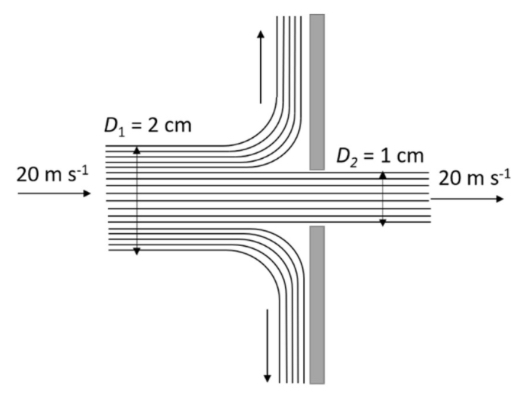
\includegraphics[width=0.5\linewidth]{figs/fig8.jpeg}
    \caption{fig8}
    \label{fig:8}
\end{figure}
\begin{enumerate} 
\begin{multicols}{4}
  \item $30\pi$
  \item $10\pi$
  \item $20\pi$
  \item $5\pi$
  \end{multicols}
  \end{enumerate}
\item Consider a horizontal road of radius aR $(a<1)$ in a stationary pipe of radius R. The rod is pulled coaxially at a constant velocity V as shown in the figure. The annual region is filled with a Newtonian incompressible fluid of viscosity $\mu$. The steady state fully developed axial velocity profile in the fluid is given by $u(r)=V \dfrac{ln(r/R)}{ln(a)}$, where r is the radial coordinate, Ignoring end effects, the magnitude of the pulling force per unit rod length is
\begin{figure}[H]
    \centering
    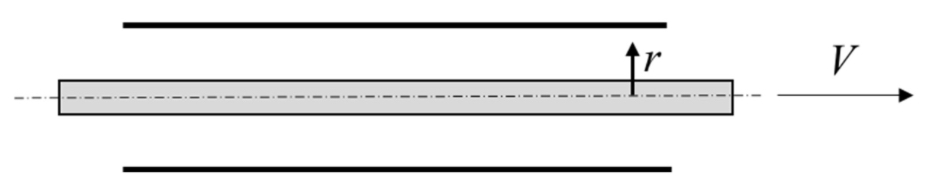
\includegraphics[width=0.5\linewidth]{figs/fig9.jpeg}
    \caption{fig9}
    \label{fig:9}
\end{figure}
\begin{enumerate} 
\begin{multicols}{4}
  \item $\pi \mu V$
  \item $-\dfrac{2\pi \mu V}{ln(a)}$
  \item $0$
  \item $-\dfrac{\pi \mu V}{ln(a)}$
  \end{multicols}
  \end{enumerate}
\item Consider a bare long copper wire of $1$ mm diameter. Its surface temperature is $T_s$ and the ambient temperature is $T_a(T_s > T_a)$. The wire is to be coated with a $2$ mm thick insulation. The convective heat transfer coefficient is $20 W m^2 K^{-1}$. Assume that  $T_s$ and $T_a$ remain unchanged. To reduce heat loss from the wire, the maximum allowed thermal conductivity of the insulating material, in $W m^{-1} K^{-1}$, rounded off to two decimal places, is
\begin{enumerate} 
\begin{multicols}{4}
  \item $0.02$
  \item $0.04$
  \item $0.10$
  \item $0.01$
  \end{multicols}
  \end{enumerate}
\newpage
\item Two large parallel planar walls are maintained at $1000$ K and $500$ K. Parallel radiation shields are to be installed between the two walls. Assume that the emissivities of the walls and the shields are equal. If the melting temperature of the shields is $900$ K, the maximum number of shield(s) that can be installed between the walls is (are)
\begin{enumerate} 
\begin{multicols}{4}
  \item $1$
  \item $0$
  \item $2$
  \item $3$
  \end{multicols}
  \end{enumerate}
  \item Saturated steam condenses on a vertical plate maintained at a constant wall temperature. If x is the vertical distance from the top edge of the plate, then the local heat transfer coefficient $h(x) \propto \Gamma(x)^{-1/3}$ where $\Gamma(x)$ is the local mass flow rate of the condensate per unit plate width. The ratio of the average heat transfer coefficient over the entire plate to the heat transfer coefficient at the bottom of the plate is
\begin{enumerate} 
\begin{multicols}{4}
  \item $4$
  \item $4/3$
  \item $3/4$
  \item $3$
  \end{multicols}
  \end{enumerate}
\item Match the product in Group-$1$ with the manufacturing process in Group-$2$. The correct combination is 
\begin{table}[h]
\centering
\begin{tabular}{|c|l|c|l|}
\hline
\textbf{Group-1} & & \textbf{Group-2} & \\ \hline
P & Nitric acid         & I   & Trona process \\ \hline
Q & Phosphoric acid     & II  & Twitchell process \\ \hline
R & Potassium chloride  & III & Ostwald's process \\ \hline
S & Stearic acid        & IV  & Haifa process \\ \hline
\end{tabular}
\end{table}
\begin{enumerate} 
\begin{multicols}{2}
  \item P-III, Q-I, R-IV, S-II
  \item P-IV, Q-I, R-II, S-III
  \item P-III, Q-IV, R-I, S-II
  \item P-I, Q-IV, R-II, S-III
  \end{multicols}
  \end{enumerate}
\item The directional derivative of $f(x,y,z)=4x^2+2y^2+z^2$ at the point $(1,1,1)$ in the direction of the vector $\bar{v}=\hat{i}-\hat{k}$ is \underline{\hspace{1.5cm}} (rounded off to two decimal places).
\vspace{0.2cm}
\item Consider a sphere of radius $4$, centered at the origin, with outward unit normal $\hat{n}$ on its surface S. The value of the surface integral $\int \int _s(\dfrac{2x\hat{i} +3y\hat{j} +4z\hat{k}}{4\pi})\hat{n} d\Lambda$ is \underline{\hspace{1.5cm}} (rounded off to one decimal place).
\vspace{0.2cm}
\item The equation $\dfrac{dy}{dx}=xy^2+2y+x-4.5$ with the initial $y(x=0)=1$ is to be solved using a predictor-corrector approach. Use a predictor based on the implicit Euler's method and a corrector based on the trapezoidal rule of integration, each with a full-step size of $0.5$. Considered only positive values of y, the value of y at $x=0.5$ is \underline{\hspace{1.5cm}} (rounded off to two decimal places).
\newpage
\item A substances at $4\degree$C has a thermal expansion coefficient $ \beta = \dfrac{1}{v} \left(\frac{\partial s}{\partial v}\right)_P= 0 K^{-1} $,an isothermal compressibility, $ \left[ K_T =-\dfrac{1}{v} \left(\frac{\partial s}{\partial v}\right)_T = 5 \times10^{-4}Pa^{-1} \right] $ and a molar volume $v=18 \times 10^{-6} m^3 mol^{-1}$. If 
s is the molar entropy, then at $4\degree$C, the quantity 
$ \left[ v \left(\frac{\partial s}{\partial v}\right)_T \right] $ evaluated for the substance is \underline{\hspace{1.5cm}}J $mol^{-1} K^{-1}$ (rounded off to the nearest integer).

\item The molar excess Gibbs free energy $(g^E)$ of a liquid mixture of A and B is given by $\dfrac{g^E}{RT}=x_A x_B [C_1+C_2(x_A-x_B)]$ where $x_A$ and $x_B$ are the mole fraction of A and B, respectively, the universal gas constant, $R=8.314J K^{-1} mol^{-1} $, T is the temperature in K and $C_1,C_2$ are temperature-dependent parameters. At $300$K, $C_1=0.45$ and $C_2=-0.018$. IF $\gamma_A$ and $\gamma_B$ are the activity coefficients of A and B, respectively, the value of $\int ^1_0ln(\dfrac{\gamma_A}{\gamma_B})dx_A$ and $300$K and $1$ bar id \underline{\hspace{1.5cm}} (rounded off to the nearest integer).

\item For a pure substance, the following data at saturated conditions are given: 
\begin{center}
\begin{tabular}{cc}

$\ln P^{\text{sat}}$ (bar) & $T$ (K) \\

0.693 & 350 \\
1.386 & 370 \\

\end{tabular}
\end{center}
Assume that the vapor phase behaves ideally, the molar volume of the liquid is negligible, and the latent heat of vaporization is constant over the given temperature range. The universal gas constant, $R=8.314 J K^{-1}mol^{-1} $. From the above data, the estimated latent heat of vaporization at 360K is \underline{\hspace{1.5cm}} kJ/mol (rounded off to one decimal place). 

\item Consider the process flowsheet in the figure. An irreversible liquid-phase reaction A $\rightarrow$ B (reaction rate $-r_A =164 x_A kmol m^{- 3}h^{- 1} $) occurs in a $1m^3$ continuous stirred tank reactor (CSTR), $x_A$ fraction of A. A small amount of inert, I, is added to the reactor. The reactor effluent is separated in a perfect splitter to recover pure B product down the bottoms and a B-free distillate. A fraction of the distillate is purged and the rest is recycled back to the reactor. At a particular steady state, the product rate is $100 kmol h^{-1}$ the recycle rate is $200 kmol h^{-1}$ and the purge rate is $10 kmol h^{-1}$ Given the above information, the inert feed rate into the process \underline{\hspace{1.5cm}} kmol $h^{-1}$ (rounded off to two decimal places).
\begin{figure}[H]
    \centering
    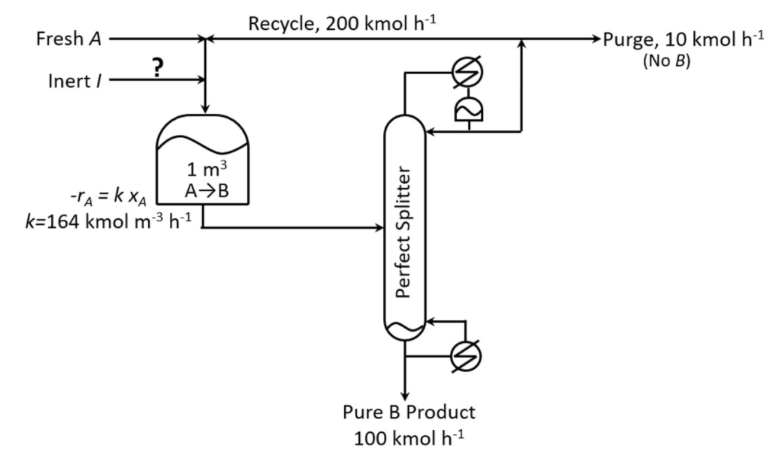
\includegraphics[width=0.5\linewidth]{figs/fig10.jpeg}
    \caption{fig10}
    \label{fig:10}
\end{figure}
\newpage
\item Two reservoirs located at the same altitude are connected by a straight horizontal pipe of length 120 m and inner diameter $0.5$ m, as shown in the figure. A pump transfers the liquid of density $800 kg m^3$ at a flow rate of $1 m^3 s^{-1}$ from Reservoir-$1$ to Reservoir-$2$. The liquid levels in Reservoir-1 and Reservoir-$2$ are $2$ m and $10$ m, respectively. Assume that the reservoirs' cross-section areas are large enough to neglect the liquid velocity at the top of the reservoirs. All minor losses can be ignored. The acceleration due to gravity is $9.8 m s^{-2} $. If the friction factor for the pipe-flow is 0.01, the required power of the pump is \underline{\hspace{1.5cm}} kW (rounded off to one decimal place).
\begin{figure}[H]
    \centering
    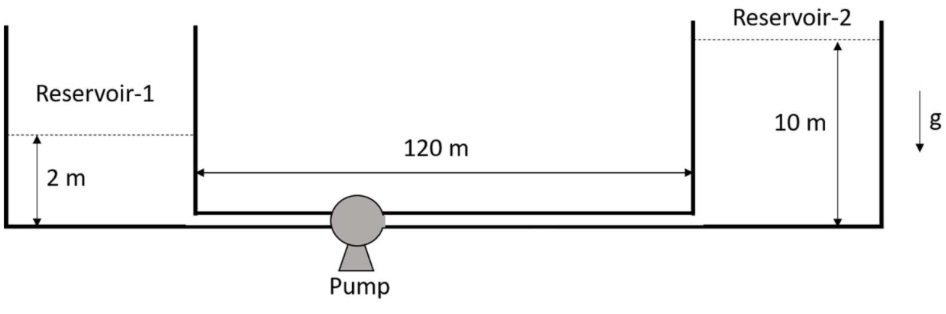
\includegraphics[width=0.6\linewidth]{figs/fig11.jpeg}
    \caption{fig11}
    \label{fig:11}
\end{figure}
\item A venturi meter (venturi coefficient, $C_v = 0.98$) is connected to a pipe of inner diameter $50$ mm. Water (density $1000 kg m^{-3}$) is flowing through the pipe. The pressure-drop measured across the venturi meter is $50$ kPa. If the venturi throat diameter is $20$ mm, the estimated flow rate of water is \underline{\hspace{1.5cm}}$\times 10 m^3 s^{-1}$ (rounded off to two decimal places).
\vspace{0.2cm}
\item In a constant-rate cake filtration operation, the collected filtrate volumes are $120 m^3$ and $240 m^3$ at $1$ min and $2$ min, respectively. Assume the cake resistance to be constant and the filter medium resistance to be negligible. If the pressure-drop across the cake is $10$ kPa at 1 min, its value at $2$ min is \underline{\hspace{1.5cm}}kPa (rounded off to the nearest integer).
\vspace{0.2cm}
\item A cylindrical fin of diameter $24$ mm is attached horizontally to a vertical planar wall. The heat transfer rate from the fin to the surrounding air is $60\%$ of the heat transfer rate if the entire fin were at the wall temperature. If the fin effectiveness is $10$, its length is \underline{\hspace{1.5cm}}mm (rounded off to the nearest integer).
\vspace{0.2cm}
\item A single-effect evaporator with a heat transfer area of $70m^2$ concentrates a salt solution using steam. The salt solution feed rate and temperature are $10000kg h ^ {- 1}$ and $40\degree$, respectively. The saturated steam feed rate and temperature are $7500 kg  h ^ {- 1}$ and $150\degree$, respectively. The boiling temperature of the solution in the evaporator is $80\degree$. The average specific heat of the solution is $0.8$ Kcal $kg^ {- 1} K ^ {- 1}$ The latent heat of vaporization is $500 Kcal kg ^ {- 1}$ If the steam-economy is $0.8$, the overall heat transfer coefficient is \underline{\hspace{1.5cm}} $kcal h^{-1}m^{-2}K^{- 1}$ (rounded off to nearest integer).
\newpage
\item An equimolar binary mixture is to be separated in a simple tray-distillation column. The feed rate is $50 k mol min^{-1}$. The mole fractions of the more volatile component in the top and bottom products are $0.90$ and $0.01$, respectively. The feed as well as the reflux stream are saturated liquids. On application of the McCabe-Thiele method, the operating line for the stripping section is obtained as $y = 1.5x - 0.005$ where y and x are the mole fractions of the more volatile component in the vapor and liquid phases, respectively. The reflux ratio is \underline{\hspace{1.5cm}} (rounded off to two decimal places).
\vspace{0.2cm}
\item The dry-bulb temperature of air in a room is $30\degree$. The Antoine equation for water is given as$ln(P ^ {rol}) = -12.00 - \dfrac{4000}{T-40}$

where T is the temperature in K and $P^{sat} $ is the saturation vapor pressure in bar. The latent heat of vaporization of water is $2000 kJ kg^{-1} $, the humid heat is $1.0 kJ kg^{-1} K^{-1} $ and the molecular weights of air and water are $28 kg kmol^{-1}$ and $18 kg kmol^{-1}$, respectively. If the absolute humidity of air is $Y'$ kg moisture per kg dry air, then for a wet-bulb depression of $9\degree, 1000 \times Y' =$ \underline{\hspace{1.5cm}} (rounded off to one decimal place).
\item In the block diagram shown in the figure, the transfer function $G=\dfrac{K}{(\tau s+1)}$ with $K>0$ and $\tau >0$. The maximum value of K below which the system remains stable is \underline{\hspace{1.5cm}} (rounded off to two decimal places).
\begin{figure}[H]
    \centering
    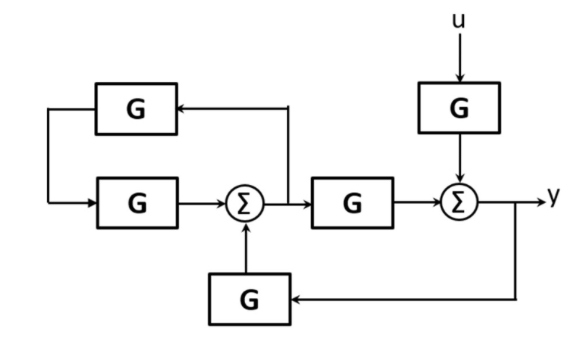
\includegraphics[width=0.3\linewidth]{figs/fig12.jpeg}
    \caption{12}
    \label{fig:12}
\end{figure}
\item Consider tank level control system shown in the figure, where the cross-section area of the tank is A. Assume perfect flow controllers (FC). The level controller (LC) is proportional-integral (PI). For an integral time,$\tau_1$. the level controller gain, $K_c$, is tuned for critical damping. The value of $\dfrac{K_c \tau_1}{A}$ is \underline{\hspace{1.5cm}} (rounded off to nearest integer).
\begin{figure}[H]
    \centering
    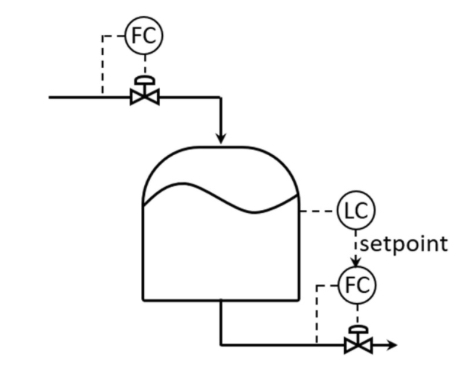
\includegraphics[width=0.3\linewidth]{figs/fig13.jpeg}
    \caption{13}
    \label{fig:13}
\end{figure}
\newpage
\item Consider a single-input-single-output (SISO) system with the transfer function $G_p(s) = \dfrac{2(s+1)}{(\dfrac{1}{2}s+1)(\dfrac{1}{4}s+1)}$ where the time constant are in minutes. The system is forced by a unit step input at time $t = 0$. The time at which the output response reaches the maximum is \underline{\hspace{1.5cm}} minutes (rounded off to two decimal places).
\vspace{0.2cm}
\item Information for a proposed greenfield project is provided in the table. The discounted cash flow for the fourth year is Rs \underline{\hspace{1.5cm}} crores (rounded off to one decimal place).
\begin{table}[H]
\centering
\begin{tabular}{cc}

Fixed capital investment (excluding land) & Rs 250 crores \\ 
Salvage value & Rs 0 \\ 
Yearly revenue from product sales & Rs 120 crores \\ 
Yearly manufacturing cost (excluding depreciation) & Rs 30 crores \\ 
Interest rate & 10\% compounded annually \\ 
Annual taxation rate & 30\% \\ 
Depreciation method & Double declining balance over seven years \\ 
Plant start-up & 2 years after project initiation \\ 

\end{tabular}
\end{table}

\textit{* $d_k = \frac{2}{7} BV_{t-1}, \; k$ years post start-up. $d$: Depreciation amount, $BV$: Book value.}
\item Consider the process in the figure. The liquid phase elementary reactions are:

\[
\begin{aligned}
&\text{A + B} \rightarrow \text{P}, \quad -r_{B1} = k_1 x_A x_B \\
&\text{P + B} \rightarrow \text{S}, \quad -r_{B2} = k_2 x_P x_B \\
&\text{S + A} \rightarrow 2\text{P}, \quad -r_{S3} = k_3 x_S x_A
\end{aligned}
\]

occur in the continuous stirred tank reactor (CSTR), where $x_i$ is the mole fraction of the $i^{\text{th}}$ component ($i = A, B, P, S$) in the CSTR. It is given that $k_2 = k_3$. All process (feed, process exit, and recycle) streams are pure. At steady state, the net generation rate of the undesired product S in the CSTR is zero. As $q = \frac{x_A}{x_B}$ is varied at constant reactor temperature, the reactor volume is adjusted to maintain a constant single-pass conversion of B. For a fixed production rate and 90\% conversion of B in the reactor, the value of $q$ that minimizes the sum of the molar flow rates of the A and S recycle streams is \_\_\_ (round off to one decimal place).
\begin{figure}[H]
    \centering
    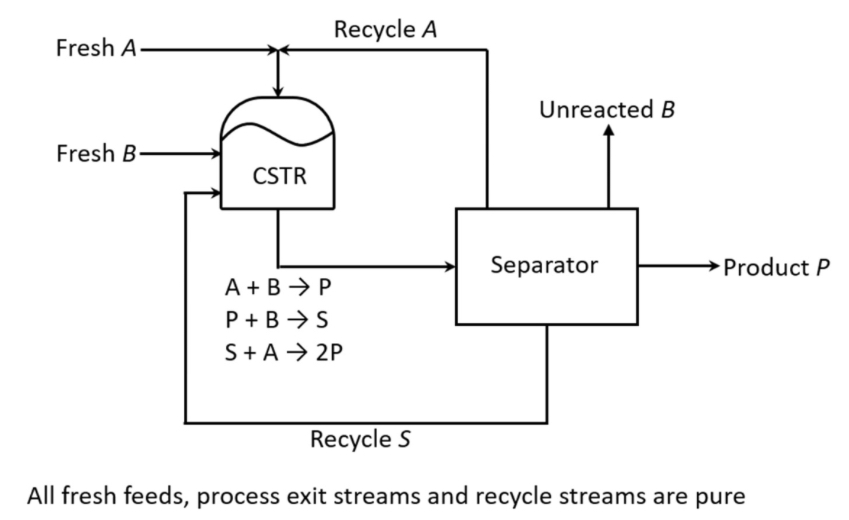
\includegraphics[width=0.4\linewidth]{figs/fig14.jpeg}
    \caption{14}
    \label{fig:14}
\end{figure}
All fresh feeds, proces exit streams and recycle streams are pure.
\newpage
\item An elementary irreversible liquid-phase reaction, 
$2A \rightarrow B$ is carried out under isothermal conditions in a $1m^3$ ideal plug flow reactor (PFR). The volumetric flow rate of fresh A is $v_1=10 m^3 h^{-1} $ and its concentration is $C_{A1} = 2 kmol m^{-3}$ For a recycle ratio $R=0$ the conversion of A with respect to the fresh feed is $50\%$. For 
$R \rightarrow \infty$, the corresponding conversion of A is \underline{\hspace{1.5cm}} $\%$(rounded off to one decimal place).
\vspace{0.2cm}
\item An elementary irreversible gas-phase reaction, 
$ A \rightarrow B + C$,is carried out at fixed temperature and pressure in two separate ideal reactors: 
(i) a $10 m^3$ plug flow reactor (PFR), (ii) a $10 m^3$ continuous-stirred tank reactor (CSTR). If pure A is fed at $5m^3h^{-1}$ to the PFR operating at $400$ K, the conversion is $80\%$. If a mixture of $50 mol\%$ of A and $50mol\%$ of an inert is fed at $5m^3 h^{-1}$ to the CSTR operating at $425$K, the conversion is $80\%$. The universal gas constant $R=8.314J mol^{-1}K^{-1} $. Assuming the Arrhenius rate law, the estimated activation energy is \underline{\hspace{1.5cm}} kJ $mol^{-1} $ (rounded off to one decimal place).
\vspace{0.2cm}
\item An elementary irreversible liquid-phase reaction, $2P \rightarrow Q$, where the rate constant $k=2Lmol^{-1} min^{-1}$, takes place in an isothermal non-ideal reactor. The E-curve in a tracer experiment is shown in the figure. Pure P $(2mol L^{-1})$ is fed to the reactor. Using the segregated model, the percentage conversion of P at the exit of the reactor is \underline{\hspace{1.5cm}}$\%$ (rounded off to nearest integer).
\begin{figure}[H]
    \centering
    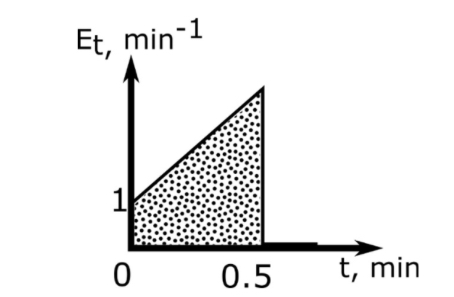
\includegraphics[width=0.5\linewidth]{figs/fig16.jpeg}
    \caption{16}
    \label{fig:16}
\end{figure}



  
\end{enumerate}
\end{document}
